\documentclass[11pt,a4paper]{article}

\usepackage[margin=2.4cm]{geometry}
\usepackage[T1]{fontenc}
\usepackage[utf8]{inputenc}
\usepackage{lmodern}
\usepackage{microtype}
\usepackage{amsmath,amssymb}
\usepackage{booktabs}
\usepackage{graphicx}
\usepackage{xcolor}
\usepackage[hidelinks]{hyperref}
\usepackage{enumitem}

\definecolor{accent}{HTML}{C85B25}
\definecolor{muted}{HTML}{555A55}
\setlength{\parindent}{0pt}
\setlength{\parskip}{0.65em}
\setlist[itemize]{leftmargin=1.4em,itemsep=2pt,topsep=3pt}

\title{AI Exposure Across Industries\\
\large A Reproducible Measurement Framework}
\author{Mario Diez Mart\'inez}
\date{Methodological appendix \textperiodcentered\ July 2026}

\begin{document}
\maketitle

\begin{abstract}
This appendix documents a reproducible pipeline for measuring artificial-intelligence exposure across US industries. It constructs two complementary measures: a direct industry score, AIIE, and a bottom-up occupational measure, ExpWB, that weights occupational AI exposure by wage-bill shares. Both are mapped through NAICS and SIC classifications into Fama--French 49 industry portfolios, aggregated using equal or BEA value-added weights, and standardized across covered portfolios. The purpose is measurement, not causal inference: exposure records the task content of an industry, not AI adoption, productivity, displacement, or realized returns.
\end{abstract}

\section{Measurement question}

Calling an industry ``AI exposed'' hides several choices. Exposure can be measured directly at the industry level or reconstructed from the occupations employed by that industry. Occupational scores can be weighted by headcount, wages, or both. Industry classifications also differ across the source data and the outcome datasets used later.

The pipeline makes each choice explicit and produces auditable variants. Its final unit is a Fama--French 49 portfolio because that classification can be joined to industry return data, but the intermediate NAICS-4 measures are retained for other labour- and real-economy applications.

\section{Data and vintages}

\begin{table}[h]
\centering
\small
\begin{tabular}{p{0.27\linewidth}p{0.20\linewidth}p{0.43\linewidth}}
\toprule
Input & Vintage & Role \\
\midrule
Felten--Raj--Seamans AIOE/AIIE & 2021 and 2023 & Occupational and direct industry AI-exposure scores; the 2023 vintage focuses on language-model capabilities. \\
BLS OEWS & May 2021 & Employment and mean annual wages by occupation-industry cell. \\
BEA GDP by Industry & 2021 & Value added used for alternative portfolio aggregation. \\
Census SIC--NAICS concordance & SIC 1987 / NAICS 2002 & Classification bridge between source industries and portfolio definitions. \\
Ken French Data Library & Current definitions & SIC ranges defining the 49 industry portfolios. \\
\bottomrule
\end{tabular}
\caption{Inputs used in the public construction pipeline.}
\end{table}

\section{Classification chain}

The mapping proceeds in two explicit steps:

\begin{enumerate}
  \item Reverse the Census SIC-to-NAICS concordance to associate each NAICS-4 industry with its candidate SIC codes.
  \item Assign each SIC code to a Fama--French portfolio and give the NAICS-4 industry the modal portfolio among its candidate SIC assignments.
\end{enumerate}

This produces a many-to-one NAICS-4-to-FF49 crosswalk. Forty-three of the 49 portfolios receive at least one valid NAICS-4 match; six remain missing and are not imputed. The public repository retains the crosswalk and aggregate mapping diagnostics.

\section{Direct industry exposure: AIIE}

Felten, Raj, and Seamans provide AI Industry Exposure scores at mixed NAICS detail. Codes are truncated to four digits, duplicate subindustry observations are averaged within NAICS-4, and the resulting industry measure is mapped to FF49.

Let $x_{i,t}^{AIIE}$ be the direct exposure of NAICS-4 industry $i$ in vintage $t\in\{2021,2023\}$. No employment or wage weights enter this first-stage score. It is therefore a direct reading of the task content assigned to the industry in the source dataset.

\section{Occupational exposure weighted by wage bill: ExpWB}

The second measure begins with occupational exposure. For occupation $o$ in industry $i$, the wage bill is

\begin{equation}
WB_{io}=L_{io}\,w_{io},
\end{equation}

where $L_{io}$ is OEWS employment and $w_{io}$ is mean annual pay. The occupation's share of the industry wage bill is

\begin{equation}
\omega_{io}=\frac{WB_{io}}{\sum_{o\in i}WB_{io}}.
\end{equation}

ExpWB is then

\begin{equation}
ExpWB_{i,t}=\sum_{o\in i}AIOE_{o,t}\,\omega_{io}
=\frac{\sum_{o\in i}AIOE_{o,t}L_{io}w_{io}}
{\sum_{o\in i}L_{io}w_{io}}.
\end{equation}

The index is dimensionless. Wage-bill weighting gives more influence to occupations that account for more employment and pay inside the industry; it does not turn exposure into a dollar loss or a forecast of automation.

\section{Portfolio aggregation}

For any NAICS-level measure $x_i$, the equal-weighted portfolio score is

\begin{equation}
x_p^{EW}=\frac{1}{N_p}\sum_{i\in p}x_i,
\end{equation}

where $N_p$ is the number of mapped NAICS-4 industries. The alternative value-added-weighted score is

\begin{equation}
x_p^{VW}=\frac{\sum_{i\in p}x_iVA_i}{\sum_{i\in p}VA_i},
\end{equation}

where $VA_i$ is 2021 BEA value added. If value added is unavailable for all industries in a portfolio, the implementation records the fallback to equal weighting rather than silently dropping the portfolio.

Every variant is standardized across portfolios with valid exposure:

\begin{equation}
z_p=\frac{x_p-\bar{x}}{s_x}.
\end{equation}

Variable names preserve the construction: measure, vintage, aggregation rule, and an optional \texttt{\_z} suffix. For example, \texttt{expwb\_23\_vw\_z} is the 2023 occupational measure aggregated with value-added weights and standardized across portfolios.

\section{Cross-measure validation}

\begin{figure}[ht]
\centering
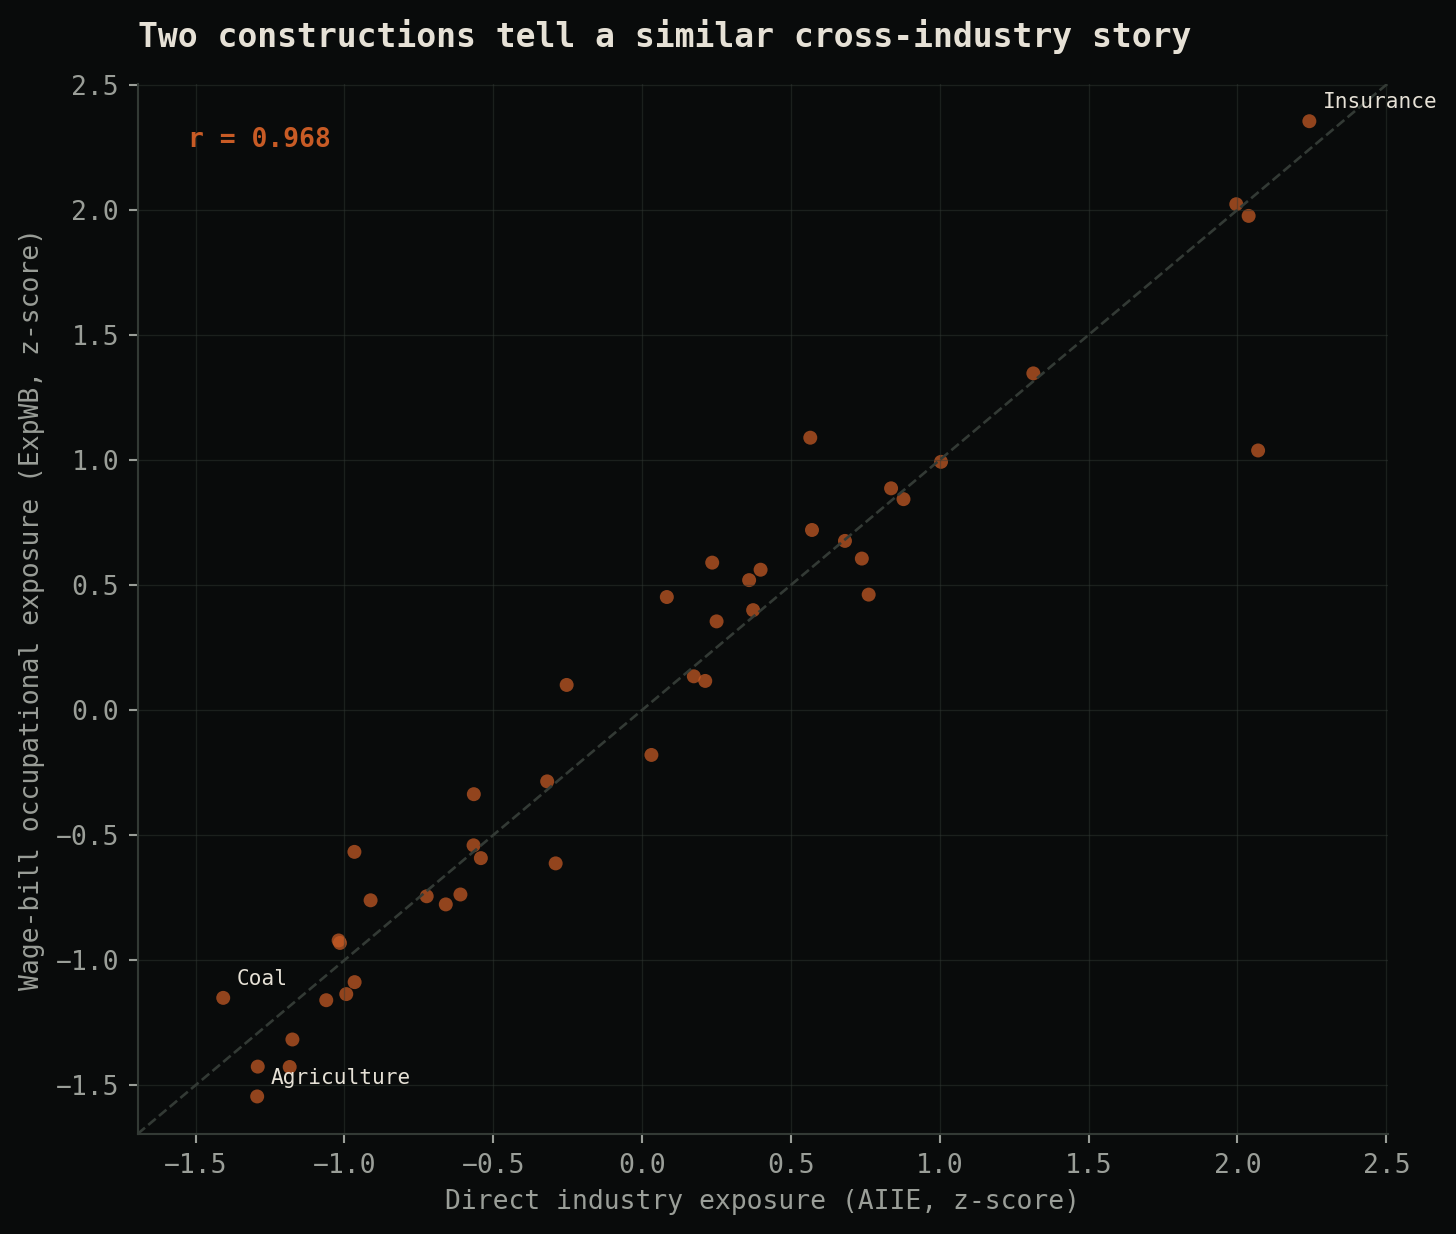
\includegraphics[width=0.91\linewidth]{../results/exposure-measure-concordance.png}
\caption{Direct industry exposure and wage-bill-weighted occupational exposure across the 43 covered Fama--French portfolios. The 2023 equal-weighted variants have correlation $r=0.968$.}
\end{figure}

The high correlation is a useful internal validation because AIIE and ExpWB reach the industry from different directions. It is not mechanical equality. Divergent portfolios remain informative: they reveal places where a direct industry classification and the occupation mix put different weight on exposure.

\begin{figure}[ht]
\centering
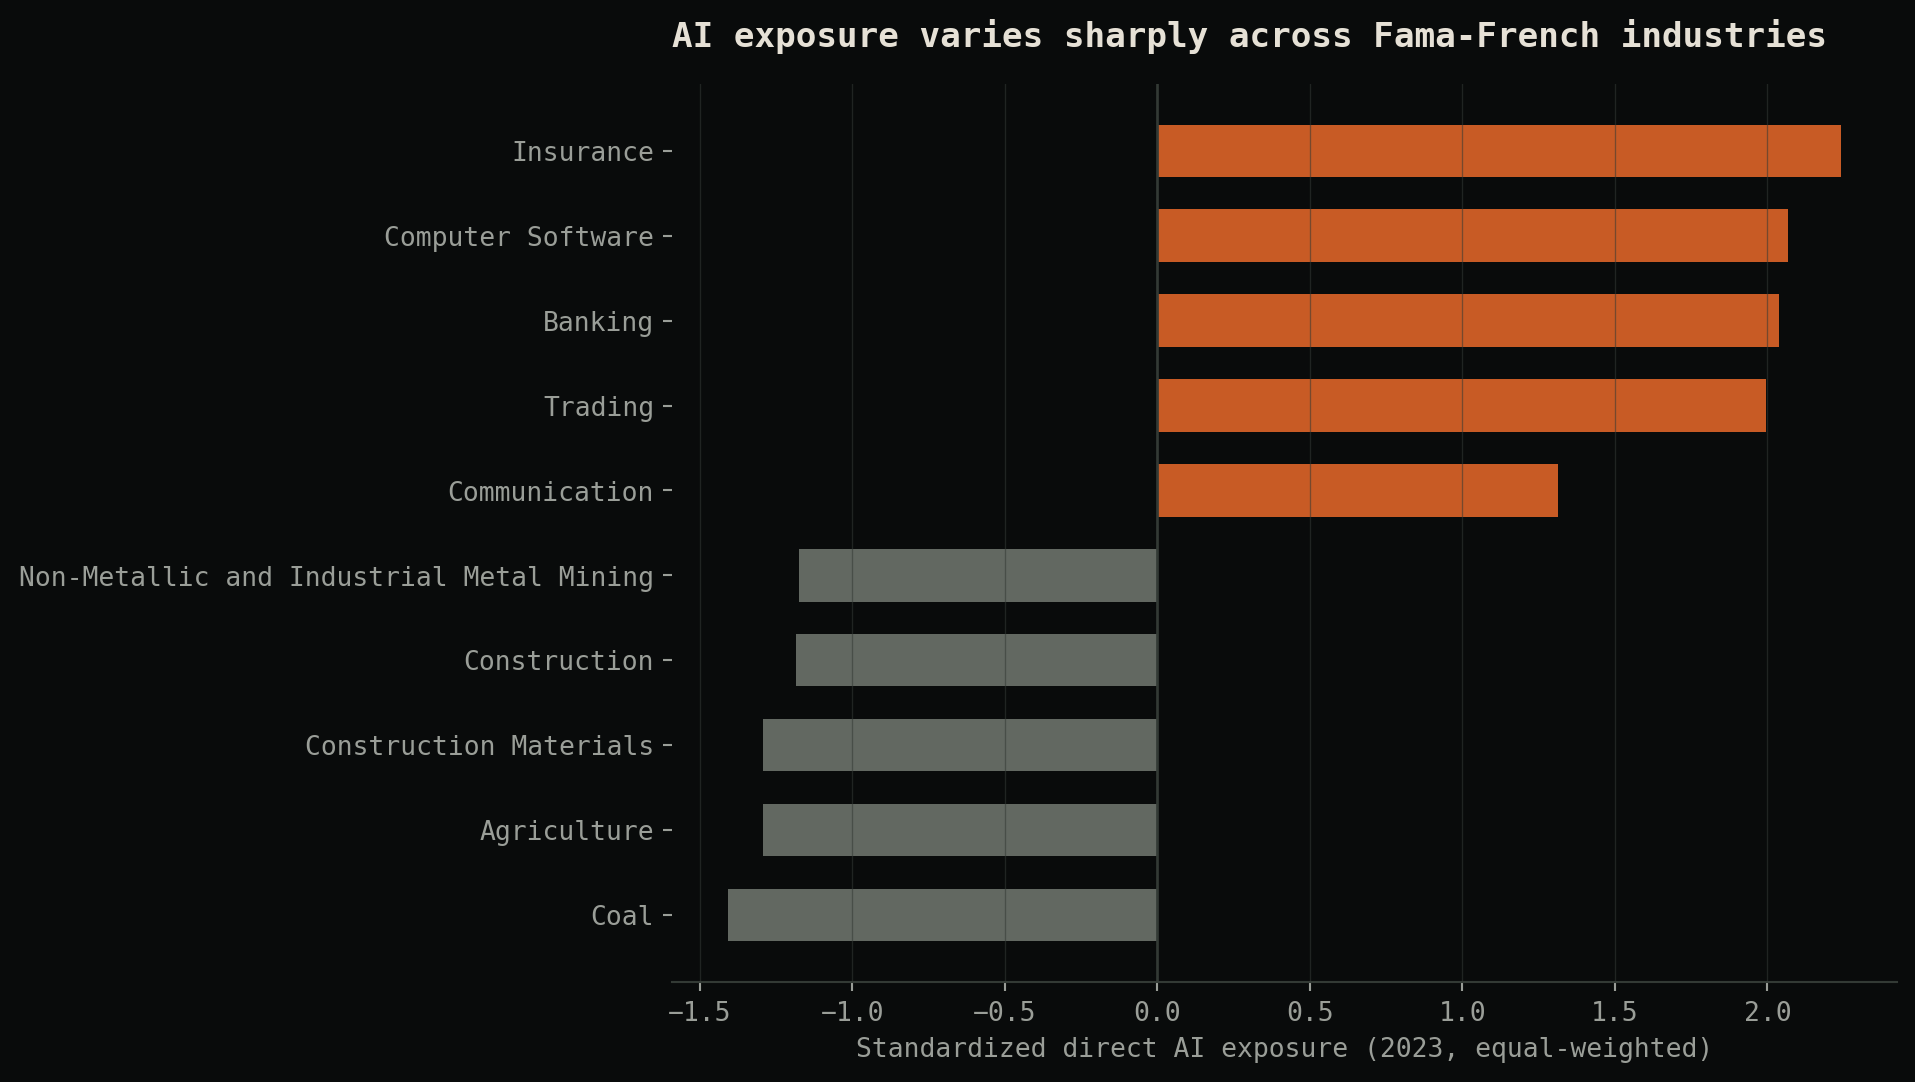
\includegraphics[width=0.96\linewidth]{../results/industry-exposure-ranking.png}
\caption{Selected high- and low-exposure portfolios using standardized 2023 equal-weighted AIIE. The chart shows relative cross-industry exposure, not adoption or economic impact.}
\end{figure}

\section{Reproducibility and boundaries}

The public release includes construction code, source adapters, the NAICS-to-FF49 mapping, NAICS-level aggregate measures, portfolio-level outputs, and figures. Reproduction requires downloading the documented public source files and supplying a personal BEA API key outside version control.

The following boundaries are intentional:

\begin{itemize}
  \item Exposure is not observed adoption, productivity, substitution, employment loss, or a causal treatment.
  \item Six FF49 portfolios are excluded rather than assigned through an unsupported match.
  \item Modal SIC assignment resolves a many-to-many concordance but can hide heterogeneous subindustries.
  \item OEWS employment and wage weights are fixed at the May 2021 vintage; occupational composition can change over time.
  \item Equal and value-added weighting answer different questions and are published side by side.
  \item Downstream return analysis remains experimental and is not part of the headline measurement claim.
\end{itemize}

\section*{References}

Felten, E., Raj, M., and Seamans, R. (2021). Occupational, Industry, and Geographic Exposure to Artificial Intelligence: A Novel Dataset and Its Potential Uses. \emph{Strategic Management Journal}, 42(12), 2195--2217.

Felten, E., Raj, M., and Seamans, R. (2023). How Will Language Modelers Like ChatGPT Affect Occupations and Industries? Working paper.

US Bureau of Labor Statistics. Occupational Employment and Wage Statistics, May 2021.

US Bureau of Economic Analysis. GDP by Industry, 2021 value-added tables.

US Census Bureau. 1987 SIC to 2002 NAICS concordance.

Kenneth R. French Data Library. Definitions of 49 Industry Portfolios.

\end{document}
